
\newpage
{\bfseries МРНТИ 44.01.81}

{\bfseries Разработка микропроцессорной системы передачи данных для
мониторинга нагрузки электроэнергетических систем}

{\bfseries \textsuperscript{1}Г.И. Жолдангарова, \textsuperscript{2,3}М.Н.
Калимолдаев, \textsuperscript{4,5}В.Б. Барахнин,
\textsuperscript{2,3}Г.З. Зиятбекова\textsuperscript{🖂},}

{\bfseries \textsuperscript{3}М.Т. Аршидинова}

\textsuperscript{1}Евразийский национальный университет имени Л.Н.
Гумилева, Астана, Казахстан,

\textsuperscript{2}Казахский национальный университет имени аль-Фараби,
Алматы, Казахстан,

\textsuperscript{3}Институт информационных и вычислительных технологий,
КН МНВО РК,

Алматы, Казахстан,

\textsuperscript{4}Федеральный исследовательский центр информационных и
вычислительных технологий, Новосибирск, Россия,

\textsuperscript{5}Новосибирский государственный университет,
Новосибирск, Россия

{\bfseries \textsuperscript{🖂}}Корреспондент-автор: ziyatbekova@mail.ru

В статье рассматривается разработка микропроцессорной системы для
мониторинга нагрузки электроэнергетических систем на основе технологий
IoT. Приведен обзор научных исследований в данной области. В качестве
пилотного прототипа разработана микропроцессорная система измерения
климатических параметров, а также напряжения и тока. Система
предназначена для обеспечения эффективного контроля и управления
тепловым насосом и связанным оборудованием. Построена информационная
схема, которая описывает взаимодействие между компонентами системы
мониторинга нагрузки электроэнергетических систем и потоки информации от
датчиков до конечного хранения данных.

{\bfseries Ключевые слова:} микропроцессорная система, датчик,
микрокомпьютер Raspberry, контроллер, платформа Arduino MEGA и FPGA.

{\bfseries ЭЛЕКТР ЭНЕРГЕТИКАЛЫҚ ЖҮЙЕЛЕРДІҢ ЖҮКТЕМЕСІН БАҚЫЛАУ ҮШІН
ДЕРЕКТЕРДІ БЕРУДІҢ МИКРОПРОЦЕССОРЛЫҚ ЖҮЙЕСІН ӘЗІРЛЕУ}

{\bfseries \textsuperscript{1}Г.И. Жолдангарова, \textsuperscript{2,3}М.Н.
Калимолдаев, \textsuperscript{4,5}В.Б. Барахнин,
\textsuperscript{2,3}Г.З. Зиятбекова\textsuperscript{🖂},}

{\bfseries \textsuperscript{3}М.Т. Аршидинова}

\textsuperscript{1}Л.Н. Гумилев атындағы Еуразия ұлттық университеті,
Астана, Қазақстан,

\textsuperscript{2}әл-Фараби атындағы Қазақ ұлттық университеті, Алматы,
Қазақстан,

\textsuperscript{3}Ақпараттық және есептеуіш технологиялар институты, ҚР
ҒК ҒЖБМ, Алматы, Қазақстан,

\textsuperscript{4}Ақпараттық және есептеу технологияларын Федералды
зерттеу орталығы,

Новосибирск, Ресей,

\textsuperscript{5}Новосибирск мемлекеттік университеті, Новосибирск,
Ресей,

е-mail: igibaevna@bk.ru

Мақалада IoT технологияларына негізделген электр энергетикалық
жүйелерінің жүктемесін бақылауға арналған микропроцессорлық жүйенің
дамуы қарастырылады. Осы саладағы ғылыми зерттеулерге шолу жасалған.
Пилоттық прототип ретінде климаттық параметрлерді, сондай-ақ кернеу мен
токты өлшейтін микропроцессорлық жүйе жасалды. Жүйе жылу сорғысымен
байланысты жабдықты тиімді бақылау мен басқаруды қамтамасыз етуге
арналған. Электр энергетикалық жүйелердің жүктемесін бақылау жүйесінің
компоненттері мен cенсорлардан деректерді соңғы сақтауға дейінгі ақпарат
ағындары арасындағы өзара әрекеттесуді сипаттайтын ақпараттық схема
құрылды.

{\bfseries Түйін сөздер:} микропроцессорлық жүйе, сенсор, Raspberry
микрокомпьютері, контроллер, Arduino Mega платформасы және FPGA.

{\bfseries DEVELOPMENT OF A MICROPROCESSOR-BASED DATA TRANSMISSION SYSTEM
FOR LOAD MONITORING OF ELECTRIC POWER SYSTEMS}

{\bfseries \textsuperscript{1}G.I. Zholdangarova, \textsuperscript{2,3}M.N.
Kalimoldayev, \textsuperscript{4,5}V.B. Barakhnin,
\textsuperscript{2,3}G.Z. Ziyatbekova\textsuperscript{🖂},}

{\bfseries \textsuperscript{3}М.Т. Arshidinova}

\textsuperscript{1}L.N. Gumilyov Eurasian National University, Astana,
Kazakhstan,

\textsuperscript{2}Al-Farabi Kazakh National University, Almaty,
Kazakhstan,

\textsuperscript{3}Institute of Information and Computational
Technologies CS MSHE RK, Almaty, Kazakhstan,

\textsuperscript{4}Federal Research Center for Information and
Computational Technologies, Novosibirsk, Russia,

\textsuperscript{5}Novosibirsk State University, Novosibirsk, Russia,

е-mail: igibaevna@bk.ru

The paper deals with the development of a microprocessor-based system
for load monitoring of electric power systems based on IoT technologies.
An overview of scientific research in the field is given. A
microprocessor-based system for measuring climatic parameters as well as
voltage and current has been developed as a pilot prototype. The system
is designed to provide effective monitoring and control of the heat pump
and related equipment. An information scheme is constructed that
describes the interaction between components of the power system load
monitoring system and the information flows from the sensors to the
final data storage system.

{\bfseries Key words:} microprocessor system, sensor, Raspberry
microcomputer, controller, Arduino MEGA and FPGA platform.

{\bfseries Введение.} Рост населения и экономики Республики Казахстан
приводит к огромному спросу на электроэнергию и энергетические ресурсы.
Как отмечают аналитики казахстанской версии журнала «Forbes», в целом по
стране наблюдается дефицит электроэнергии, что делает энергетический
сектор уязвимым. Казахстан столкнулся с дефицитом электрической энергии
и мощности, который в вечерние часы составляет более 1,3 ГВт. В
региональном же разрезе, особенно в южной зоне, дефицит электроэнергии
серьёзно подрывает энергетическую безопасность страны. Только в марте
2023 года в Южном Казахстане производство компенсировало всего 57,2\%
потребления --- дефицит составил 971,0 млн кВт·ч.

В сложившихся условиях важно иметь инструмент для мониторинга нагрузки в
энергосистеме с целью выявления на его основе возможного развития
критических ситуаций, чтобы иметь возможность принимать управленческие
решения для недопущения их возникновения. Эффективным методом решения
данной задачи является использования технологий Интернета вещей (IoT)
для мониторинга процессов в энергосистеме {[}1{]}, сочетающего в себе
несколько методов анализа и прогнозирования данных о потреблении
электроэнергии {[}2{]}.

Использование IoT в энергетическом секторе относится к числу бурно
развивающихся в настоящее время технологий. Нашим вкладом в развитие
этой области будет разработка встроенного контроллера Arduino MEGA и
FPGA. Все критические параметры на подстанции, включая напряжение,
частоту, мощность, состояние выключателя и температуру внутри системы,
контролируются с его использованием посредством занесения в базу данных
веб-сервера для последующего анализа. Предопределенные механизмы запуска
событий также запрограммированы на контроллере с функциями записи:
данные записываются контроллером и передаются на веб-сервер с помощью
микроконтроллера ESP32. Контроллер, встроенный в FPGA, обеспечивает
высокоскоростные и надежные функции сбора и обработки данных.

Информационные системы имеют преимущества по сравнению с традиционными
методами мониторинга. Они способны выявлять сложные закономерности в
данных, что повышает точность прогнозов. В целом разработка этой
информационной системы открывает перспективы для повышения надежности и
эффективности энергосистем.

Стратегической целью этой программы является разработка информационной
системы для мониторинга нагрузки электроэнергетических сетей на основе
IoT-технологий, использующих встроенный контроллер Arduino MEGA и FPGA
для мониторинга на подстанции напряжения, частоты, мощности, состояния
выключателя, температуры внутри системы.

Микропроцессорная система включает в себя следующие компоненты:

\begin{itemize}
\item
  Модуль сбора данных: Сбор данных о нагрузке и других параметрах сети с
  помощью датчиков IoT.
\item
  Модуль очистки данных: Предварительная обработка данных для удаления
  шумов и выбросов.
\item
  Модуль представления результатов: Формирование отчетов и визуализация
  результатов прогнозирования.
\end{itemize}

{\bfseries Литературный обзор.} Интернет вещей (IoT) стал революционной
технологией в области мониторинга энергосетей {[}3, 4{]}. Благодаря
решению проблем и использованию возможностей FPGA продолжит
трансформировать энергетический сектор {[}5{]}. B {[}6, 7, 8{]} статьи
охватывают широкий спектр тем, включая приложения IoT для мониторинга
нагрузки, преимущества и проблемы использования IoT, а также будущие
направления развития в Республике Казахстан.

Прежде всего, отметим статью {[}8{]} академика М.Н. Калимолдаева,
которая вносит весомый вклад в разработку информационных систем с
интегрированными модулями машинного обучения для робототехники и
автоматизации. Идеи этой статьи получают дальнейшее развитие в данной
работе. Направление исследований определяется тем, что Интернет вещей в
последнее время приобрел широкое распространение. Так в статье {[}9{]}
представлен подход на основе Интернета вещей к решению проблем
энергетики.

Данное исследование реализовано для удовлетворения этих потребностей
путем разработки нового интеллектуального датчика FPGA. Указанный подход
для решения различных задач описан в работах {[}10, 11, 12, 13, 14{]}.

Многократное выполнение прикладной программы отнимает огромное
количество времени. Чтобы сократить время выполнения, в статье {[}15{]}
предлагается использовать адаптивную модель.

Автор в {[}16{]} предположил, что использование технологии Fog/Edge
может обеспечить решение таких проблем, как осуществимость Интернета
вещей (соображения безопасности в отношении вычислений и стоимости
системы) и будущая осуществимость (надлежащее проектирование
инфраструктуры для будущих приложений).

Управление электроприборами включает в себя сбор и анализ данных об их
энергопотреблении, оптимизацию графиков их работы, расчет показателей
энергопотребления и реализацию решений по оптимизации энергопотребления
{[}17{]}.

Статьи {[}18, 19, 20, 21{]} содержат ценную информацию об использовании
Интернета вещей для повышения эффективности и надежности
электроэнергетических сетей посредством мониторинга нагрузки.

Вот некоторые ключевые выводы из этих статей:

- Технологии Интернета вещей могут значительно повысить точность
мониторинга и прогнозирования нагрузки.

- Системы на базе Интернета вещей могут собирать данные в режиме
реального времени из широкого спектра источников, которые можно
использовать для разработки более точных моделей нагрузки.

- Системы на базе Интернета вещей можно использовать для выявления
событий экстремальной нагрузки, что может помочь предотвратить перебои в
подаче электроэнергии.

- Системы на базе Интернета вещей можно использовать для оптимизации
энергопотребления, что может помочь снизить затраты и воздействие на
окружающую среду.

{\bfseries Материалы и методы.} Рассмотрена методика экспериментальных
исследований, описан процесс обработки результатов измерения.

{\bfseries Результаты и дискуссия.}

\emph{Этап 1. Для начального этапа, разработки умной системы для
мониторинга электропотребления,} уровни Технологической Готовности (TRL)
могут быть описаны следующим образом:

\begin{itemize}
\item
  теоретическое исследование возможностей интеграции датчиков IoT и
  интеллектуальных счетчиков;
\item
  разработка и тестирование первичных версий системы с использованием
  реальных данных в лабораторных условиях;
\item
  анализ данных и предоставление информации о потреблении электроэнергии
  пользователям.
\end{itemize}

Каждый этап TRL требует определенных исследований, разработок и
тестирований, а также постепенного увеличения масштаба и их сложности.
Это обеспечивает систематический подход к разработке и внедрению
технологии.

\emph{Этап 2. Разработка высокоскоростной системы сбора и обработки
данных контроллера.}

На втором этапе контроллер, встроенный в FPGA, обеспечивает
высокоскоростной и надежный сбор и обработку данных. Сбор данных
осуществляется с помощью датчиков Zmpt101b и ACQ720. Благодаря высокой
частоте дискретизации системы как установившиеся, так и переходные
режимы энергосистемы контролируются с использованием одного источника
времени. С помощью платформы IoT данные передаются через локальную сеть
для записи в базу данных. Критерием успешной реализации будет точность,
надежность и производительность системы.

Технологическая готовность определяется наличием высокоскоростной
системы сбора и обработки данных контроллера в составе
полнофункционального макета информационной системы мониторинга нагрузки
электроэнергетических сетей -- индекс готовности {[}22, 23{]}.

\emph{Этап 3. Разработка методов и протоколов связи, а также необходимых
мер кибербезопасности для занесения на сервер данных встроенного
контроллера Arduino MEGA и FPGA.}

Основными принципами исследования являются существующие технологии и
методы передачи данных и кибербезопасности. Теоретическая разработка
концепции протоколов связи и мер кибербезопасности для Arduino MEGA и
FPGA.

TRL включает в себя углубление исследований, разработок и тестирований,
обеспечивая поэтапный и систематический подход к разработке и внедрению
технологии в реальные условия.

\begin{figure}[H]
	\centering
	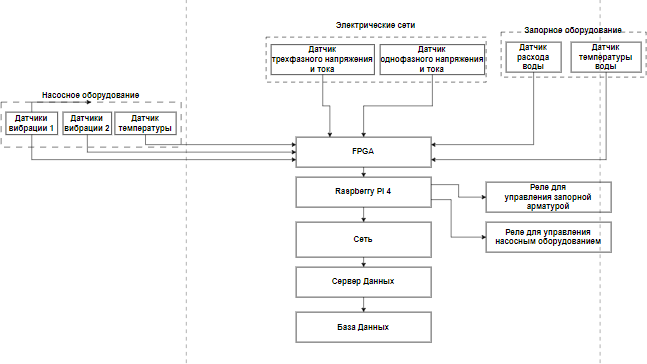
\includegraphics[width=0.8\textwidth]{assets/148}
	\caption*{\bfseries Рис. 1 - Структурная схема системы}
\end{figure}


Опишем пилотный прототип создаваемой системы, предназначенный для
обеспечения эффективного контроля и управления тепловым насосом и
связанным оборудованием, основная задача которого -- сбор данных от
датчиков, их обработка и использование для управления насосом и запорной
арматурой в реальном времени. Информационная схема описывает
взаимодействие между компонентами системы и потоком информации от
датчиков до конечного хранения данных (Рисунок 1).

\emph{Описание компонентов и их взаимодействия}

\emph{Датчики:}

\begin{itemize}
\item
  Датчики вибрации 1 и 2 устанавливаются на корпусе насоса и ближе к
  ротору, чтобы измерять вибрации, которые могут указывать на возможные
  механические неисправности или износ.
\item
  Датчик температуры монтируется на корпусе насоса рядом с подшипниками,
  отслеживая его рабочую температуру для предотвращения перегрева.
\item
  Датчик трёхфазного напряжения и тока измеряет параметры трехфазных
  цепей, что позволяет контролировать (для мониторинга) нагрузку и
  напряжение.
\item
  Датчик однофазного напряжения и тока контролирует однофазные цепи,
  обеспечивая дополнительную информацию о состоянии системы.
\item
  Датчик расхода воды измеряет объем или поток воды, проходящей через
  насос, чтобы обеспечить его оптимальную работу и предотвратить
  возможные проблемы.
\item
  Датчик температуры воды контролирует температуру воды в системе, что
  важно для управления процессами и предотвращения перегрева.
\end{itemize}

\emph{Сбор данных:} Все датчики передают данные на Raspberry Pi 4 через
FPGA, который выполняет первичную обработку всех данных (вибрации,
температуры, напряжения и тока), т.е. регулярно отправляют свои
показания.

\emph{Устройства управления:}

\begin{itemize}
\item
  Реле для управления запорной арматурой управляет клапанами и запорной
  арматурой в системе, контролируя потоки жидкости и обеспечивая их
  правильное направление.
\item
  Реле для управления насосом включает/выключает насос в зависимости от
  условий работы, заданных в программном обеспечении Raspberry Pi 4. Это
  позволяет автоматически регулировать работу насоса в ответ на
  изменения в системе. Raspberry Pi 4 отправляет команды на реле для
  управления насосом и запорной арматурой, основываясь на полученных
  данных и выполненном анализе.
\end{itemize}

Команды управления реле (для запорной арматуры и насоса) формируются на
основе данных от датчиков и логики управления.

\emph{FPGA:}

\begin{itemize}
\item
  FPGA получает данные от всех датчиков (вибрация, температура,
  трехфазное и однофазное напряжение и ток).
\item
  Выполняет первичную обработку данных, включая фильтрацию и
  сглаживание.
\item
  Обработанные данные передаются на Raspberry Pi 4.
\end{itemize}

\emph{Контроллер:}

\begin{itemize}
\item
  Raspberry Pi 4 (центральный контроллер системы)
\end{itemize}

Платформа IoT основана на базе Raspberry Pi 4, которая является основной
в системе и необходима для обработки данных; управления реле и передачи
данных через сеть. Данные могут быть переданы на сервер для хранения и
анализа. Сервер базы данных принимает данные от платформы IoT и
сохраняет их для дальнейшего отображения в ситуационном центре, анализа
и отчетности.

Raspberry Pi 4 и FPGA выступает в роли центрального контроллера системы.
Они принимают данные от всех датчиков через соответствующие интерфейсы
(GPIO, SPI, I2C или USB). Raspberry Pi 4 обрабатывает данные, выполняет
вычисления и принимает решения на основе предустановленных алгоритмов.

\emph{Обработка данных:} Raspberry Pi 4 через FPGA получает данные от
датчиков, обрабатывает их в реальном времени, используя установленные
алгоритмы и логические правила. На основе анализа данных принимаются
решения о необходимости включения или выключения насосов и управления
запорной арматурой.

\emph{Интерфейсы и связи:}

\begin{itemize}
\item
  Интерфейсы датчиков (например, аналоговые выходы, цифровые сигналы)
\item
  SPI/I2C/USB (интерфейсы для подключения датчиков и реле к Raspberry Pi
  4)
\item
  Ethernet/Wi-Fi (для передачи данных в локальную сеть)
\end{itemize}

\emph{Платформа IoT:}

\begin{itemize}
\item
  Локальная сеть (LAN)
\item
  Сервер данных (для хранения и обработки данных)
\end{itemize}

Данные от Raspberry Pi 4 передаются в локальную сеть (LAN) через
Ethernet или Wi-Fi. Платформа IoT в сети обеспечивает связь между
Raspberry Pi 4 и сервером данных. Сервер данных принимает и хранит
данные, переданные от Raspberry Pi 4. Это может включать в себя хранение
исторических данных, обработку информации и выполнение аналитики.

\emph{База данных:}

Сервер базы данных (например, SQL или NoSQL база данных для хранения
данных). База данных на сервере служит для долговременного хранения
данных. Здесь сохраняются все данные, полученные от датчиков и
обработанные контроллером. База данных также используется для
формирования отчетов и анализа состояния системы. Обработанные данные
передаются в локальную сеть, затем на сервер данных, где сохраняются в
базе данных. Данные могут быть использованы для последующего анализа,
формирования отчетов и оптимизации работы системы.

\emph{Реляционная база данных (SQL). Форматы и таблицы:}

\emph{Таблица sensor\_data:}

\begin{itemize}
\item
  id (INT, PK) --- Уникальный идентификатор записи
\item
  timestamp (TIMESTAMP) --- Время измерения
\item
  sensor\_type (VARCHAR) --- Тип датчика (вибрация, температура,
  напряжение и т.д.)
\item
  sensor\_location (VARCHAR) --- Местоположение датчика (например,
  корпус насоса, ротор и т.д.)
\item
  value (FLOAT) --- Значение измерения
\end{itemize}

\emph{Таблица device\_control:}

\begin{itemize}
\item
  id (INT, PK) --- Уникальный идентификатор записи
\item
  timestamp (TIMESTAMP) --- Время управления
\item
  device\_type (VARCHAR) --- Тип устройства (например, насос, запорная
  арматура)
\item
  action (VARCHAR) --- Действие (включить/выключить)
\end{itemize}

\emph{Таблица system\_logs:}

\begin{itemize}
\item
  id (INT, PK) --- Уникальный идентификатор записи
\item
  timestamp (TIMESTAMP) --- Время события
\item
  log\_type (VARCHAR) --- Тип лога (ошибка, предупреждение и т.д.)
\item
  message (TEXT) --- Сообщение лога
\end{itemize}

\emph{Преимущества:}

\begin{itemize}
\item
  Хорошо структурированы данные.
\item
  Поддержка сложных запросов и транзакций.
\item
  Хорошая поддержка для аналитики и отчетности.
\end{itemize}

Приступим к описанию разрабатываемой система мониторинга
электропотребления. Предлагается следующая ее схема, состоящая из трех
блоков:

1) блок приема и передачи текущей информации (вибрации, температуры,
напряжения и тока);

2) блок обработки постоянной и оперативной информации об угрозе аварии
(сервер);

3) блок прогнозирования аварийных ситуаций в энергосистемах.

Основной информацией для мониторинга нагрузки электроэнергетических
систем являются данные, поступающие от датчиков, показанных на рисунке
1. Дополнительную информацию дают данные с датчиков через
соответствующие интерфейсы. Блок приема-передачи текущей информации
реализован в виде датчиков вибрации, температуры, напряжения и тока.
Датчики подключены к микропроцессору Arduino, который обеспечивает
предварительную обработку поступающих с датчиков данных и передает их
для дальнейшей обработки. Используется устройство на базе
микроконтроллера ATmega 328. В комплект поставки входит все необходимое
для удобной работы с микроконтроллером. Для начала работы с устройством
достаточно подать питание от адаптера переменного/постоянного тока или
аккумулятора, либо подключить его к компьютеру с помощью USB-кабеля.

Блок обработки постоянной и оперативной информации об угрозе аварийных
ситуаций содержит постоянную информацию о характеристиках энергосистемы,
а также оперативно получает текущую информацию, на основе обработки
которой блок рассчитывает уровень безопасности, тревожности или
катастрофичности электроэнергетического комплекса. В последнем случае он
автоматически оповещает государственные органы (МЧС, акиматы и т.д.) о
возможной угрозе аварии.

{\bfseries Выводы.} В целом использование Интернета вещей для мониторинга
нагрузки электроэнергетических сетей является быстро развивающейся
областью исследований, которая потенциально может оказать существенное
влияние на энергетический сектор.

Дано описание разработанной в Казахстане технологии мониторинга нагрузки
электроэнергетических систем, обсуждены результаты ее практического
использования в отдельных регионах и намечены направления дальнейшего
развития. Сформулированы цель и основные задачи исследований,
направленных на разработку методики прогнозирования
электроэнергетической аварии как чрезвычайной ситуации на основе анализа
различных существующих методов. Использован метод непрерывной волны или
метод ультразвукового импульсного эха. В качестве пилотного прототипа
разработана автономная микрокомпьютерная система передачи климатических
данных на основе микропроцессорной техники и датчиков. Разработана
программа мониторинга факторов волн нагрузки в режиме реального времени
для датчиков определения уровня безопасности.

\emph{{\bfseries Финансирование.}} Работа выполнена за счет средств
грантового финансирования научных исследований на 2024-2026 годы по
проекту АР23490529 «Разработка информационной системы и математических
моделей для мониторинга и прогнозирования нагрузки электроэнергетических
систем на основе гибридных технологий».

{\bfseries Литература}

1.Ahmed N., De D., Hussain M. I. Internet of things (IoT) for smart
precision agriculture and farming in rural areas // IEEE Internet of
Things Journal. 2018. Vol. 5(6)- P. 4890- 4899.

DOI 10.1109/JIOT.2018.2879579

2. Liangzhi Li, Kaoru Ota, Mianxiong Dong. When Weather Matters:
IoT-Based Electrical Load Forecasting for Smart Grid // IEEE
Communications Magazine, 2017. -- Vol. 5(10).- P. 46-51. DOI
10.1109/MCOM.2017.1700168

3.Prasanna Hambarde, Rachit Varma, Shivani Jha. The Survey of Real Time
Operating System: RTOS. -- IEEE International Conference on Electronic
Systems, Signal Processing and Computing Technologies, 2014. DOI
10.1109/ICESC.2014.15

4. Kalimoldayev M., Akhmetzhanov М., Kunelbayev М., Sundetov Т.
Information systems of integrated machine learning modules on the
example of a verbal robot // News of the National Academy of sciences of
the Republic of Kazakhstan. Series of geology and technical sciences,
2019. -No. 6(438).- P. 215-222. DOI 10.32014/2019.2518-170X.173

5.Kalimoldayev M., Tynymbayev S., Magzom M., Tananova D., Lyshevski S.
FPGA Implementation of Encryption Algorithms Based on Residual
Polynomials // 2020 IEEE 40th International Conference on Electronics
and Nanotechnology (ELNANO), IEEE, Kyiv, Ukraine, 2020. DOI
10.1109/ELNANO50318.2020.9088890

6.Kalimoldayev M., Akhmetzhanov M., Kunelbayev M. Determination of the
power interaction of the hydro turbine GRID with a fluid flow for a
double-rotor micro hydro power plant // Известия НАН РК. Серия
физико-математическая, 2019. -- No. 4. -- P. 59-67.

DOI 10.32014/2019.2518-1726.4

7.Kalimoldayev M., Akhmetzhanov M., Kunelbayev M. Development and
research of a mathematical model of a solar photo converter with an
inverter for converting direct current to alternating voltage //
Известия НАН РК. Серия физико-математическая, 2019. -- No. 4. -- P.
135-142. DOI 10.32014/2019.2518-1726.52

8.Kalimoldayev M.N., Pak I. T.,Baipakbayeva S., Mun G., Shaltykova D.
B., I. E. Suleimenov

Methodological basis for the development strategy of artificial
intelligence systems in the Republic of Kazakhstan in the message of the
president of the Republic of Kazakhstan // News of the National Academy
of Sciences of the Republic of the Kazakhstan. Series of geology and
technical sciences, 2018. -- Vol. 6. -- P. 47-54. DOI
10.32014/2018.2518-170X.34

9.Kalimoldayev M.N., Abdildayeva A., Zhukabayeva T., Turaev Sh. The
investigation of the

internet of things (IoT) in electric power systems // News of the
National Academy of Sciences of the Republic of Kazakhstan. Series of
Geology and Technical Sciences, 2019. -- Vol. 5. -- No. 437. -- P.
144-150. DOI 10.32014/2019.2518-170X.136

10.{[}online{]} Available: http://www.ni.com/fpga/ (17.07.2024)

11.Introduction to FPGA technology: Top 5 benefits, {[}online{]}
Available: http://www.ni.com/white-paper/6984/en/ (13.05.2024)

12.Hao Z., Lianping G., Jie M., and Peng Y. Research on the hardware
co-processing technology for waveform character searching with a digital
oscilloscope, Proc. 13th IEEE Int. Conf. Electron. Meas. Instrum,
2017.-P. 92-97. DOI 10.1109/ICEMI.2017.8265920

13.Escobar F.A., Chang X., and Valderrama C. Suitability analysis of
FPGAs for heterogeneous platforms in HPC, IEEE Trans. -- Parallel
Distrib. Syst. 2016, -- Vol. 27(2). -- P. 600-612.

DOI 10.1109/TPDS.2015.2407896

14.Sheng J., Yang C., Sanaullah A., Papamichael M., Caulfield A., and
Herbordt M.C. HPC on FPGA clouds: 3D FFTs and implications for molecular
dynamics, 2017. -- Proc. 27th Int. Conf. Field Program. Logic Appl. DOI
10.23919/FPL.2017.8056853

15.Chen R., and Prasanna V.K. Computer generation of high throughput and
memory efficient sorting designs on FPGA, IEEE Trans. -- Parallel
Distrib. Syst. 2017. -- Vol. 28. -- No. 11. -- P. 3100-3113.
DOI:~10.1109/TPDS.2017.2705128

16.Хироаки Н. Information and communication platform for providing smart
community services: System implementation and use case in Saitama city
// Proceedings of the IEEE International Conference on Industrial
Technology, 2018. -- Р. 1375-1380. DOI 10.1109/ICIT.2018.8352380.

17.Hussien N. Ali, Daleh Al-Magsoosi A.A., AlRikabi S., Abed F.T.
Monitoring the Consumption of Electrical Energy Based on the Internet of
Things Applications // International Journal of Interactive Mobile
Technologies.- 2021.-Vol.15(07). DOI 10.3991/ijim.v15i07.20183.

18.Motlagh N.H., Mohammadrezaei M., Hunt J., Zakeri B. Internet of
Things (IoT) and the Energy Sector // Energies, 2020.
DOI:10.3390/en13020494

19.Liu Hua, Junguo Zhang, Lin Fantao. Internet of Things Technology and
its Applications in Smart Grid // TELKOMNIKA Indonesian Journal of
Electrical Engineering.- 2014.-Vol. 12. (2)- DOI
10.11591/telkomnika.v12i2.4178

20.Tanveer Ahmad, Dongdong Zhang. Using the internet of things in smart
energy systems and networks //Sustainable Cities and Society.-
2021.-Vol. 68. DOI 10.1016/j.scs.2021.102783

21.Mohammad Kamrul Hasan, Musse Mohamud Ahmed, Bishwajeet Pandey, Hardik
Gohel, Shayla Islam, Izzul Fitrie Khalid. Internet of Things-Based Smart
Electricity Monitoring and Control System Using Usage Data // Wireless
Communications and Mobile Computing.- 2021.

- P.1-16/ DOI 10.1155/2021/6544649

21.Suryanarayanan A., Ramamurthy A., Chaudhry A.K. Internet of Things
for monitoring and forecasting the load Electric Power Networks: Future
Directions. IEEE Access Journal, 2021. -- Vol. 9. -- Pp. 136350-136379

22.Chen C., Li K., Duan M. Chapter 6. Extreme Learning Machine and Its
Applications in Big Data Processing. Big Data Analytics for
Sensor-Network Collected Intelligence Intelligent Data-Centric Systems,
2017. -- Pp. 117-150. https://doi.org/10.1016/B978-0-12-809393-1.00006-4

23.Heddam S., Kim S., Mehr A., Zounemat-Kermani M. Chapter 11. A long
short-term memory deep learning approach for river water temperature
prediction. Current Trends and Advances in Computer-Aided Intelligent
Environmental Data Engineering Intelligent Data-Centric Systems, 2022. -
P. 243-270. https://doi.org/10.1016/B978-0-323-85597-6.00015-X.

{\bfseries References}

1.Ahmed N., De D., Hussain M. I. Internet of things (IoT) for smart
precision agriculture and farming in rural areas // IEEE Internet of
Things Journal. 2018. Vol. 5(6)- P. 4890- 4899.

DOI 10.1109/JIOT.2018.2879579

2. Liangzhi Li, Kaoru Ota, Mianxiong Dong. When Weather Matters:
IoT-Based Electrical Load Forecasting for Smart Grid // IEEE
Communications Magazine, 2017. -- Vol. 5(10).- P. 46-51. DOI
10.1109/MCOM.2017.1700168

3.Prasanna Hambarde, Rachit Varma, Shivani Jha. The Survey of Real Time
Operating System: RTOS. -- IEEE International Conference on Electronic
Systems, Signal Processing and

Computing Technologies, 2014. DOI 10.1109/ICESC.2014.15

4. Kalimoldayev M., Akhmetzhanov М., Kunelbayev М., Sundetov Т.
Information systems of integrated machine learning modules on the
example of a verbal robot // News of the National Academy of sciences of
the Republic of Kazakhstan. Series of geology and technical sciences,
2019. -No. 6(438).- P. 215-222. DOI 10.32014/2019.2518-170X.173

5.Kalimoldayev M., Tynymbayev S., Magzom M., Tananova D., Lyshevski S.
FPGA Implementation of Encryption Algorithms Based on Residual
Polynomials // 2020 IEEE 40th International Conference on Electronics
and Nanotechnology (ELNANO), IEEE, Kyiv, Ukraine, 2020. DOI:
10.1109/ELNANO50318.2020.9088890

6.Kalimoldayev M., Akhmetzhanov M., Kunelbayev M. Determination of the
power interaction of the hydro turbine GRID with a fluid flow for a
double-rotor micro hydro power plant // Izvestiya NAN RK. Seriya
fiziko-matematicheskaya, 2019. -- No. 4. -- P. 59-67.
DOI10.32014/2019.2518-1726.4

7.Kalimoldayev M., Akhmetzhanov M., Kunelbayev M. Development and
research of a mathematical model of a solar photo converter with an
inverter for converting direct current to alternating voltage //
Izvestiya NAN RK. Seriya fiziko-matematicheskaya, 2019. -- No. 4. -- P.
135-142. DOI 10.32014/2019.2518-1726.52

8.Kalimoldayev M.N. Methodological basis for the development strategy of
artificial intelligence systems in the Republic of Kazakhstan in the
message of the president of the Republic of Kazakhstan // News of the
National Academy of Sciences of the Republic of the Kazakhstan. Series
of geology and technical sciences, 2018. -- Vol. 6. -- P. 47-54.
DOI10.32014/2018.2518-170X.34

9.Kalimoldayev M.N. The investigation of the internet of things (IoT) in
electric power systems // News of the National Academy of Sciences of
the Republic of Kazakhstan. Series of Geology and Technical Sciences,
2019. -- Vol. 5. -- No. 437. -- P. 144-150. DOI
10.32014/2019.2518-170X.136

10.{[}online{]} Available: http://www.ni.com/fpga/ (17.07.2024)

11.Introduction to FPGA technology: Top 5 benefits, {[}online{]}
Available: http://www.ni.com/white-paper/6984/en/ (13.05.2024)

12.Hao Z., Lianping G., Jie M., and Peng Y. Research on the hardware
co-processing technology for waveform character searching with a digital
oscilloscope, Proc. 13th IEEE Int. Conf. Electron. Meas. Instrum, 2017.
-- P. 92-97. DOI 10.1109/ICEMI.2017.8265920

13.Escobar F.A., Chang X., and Valderrama C. Suitability analysis of
FPGAs for heterogeneous platforms in HPC, IEEE Trans. -- Parallel
Distrib. Syst. 2016, -- Vol. 27. --No. 2. -- P. 600-612.

DOI 10.1109/TPDS.2015.2407896

14.Sheng J., Yang C., Sanaullah A., Papamichael M., Caulfield A., and
Herbordt M.C. HPC on FPGA clouds: 3D FFTs and implications for molecular
dynamics, 2017. -- Proc. 27 th Int. Conf. Field Program. Logic Appl.

15.Chen R., and Prasanna V.K. Computer generation of high throughput and
memory efficient sorting designs on FPGA, IEEE Trans. -- Parallel
Distrib. Syst. 2017. -- Vol. 28. -- No. 11. -- P. 3100-3113. DOI
10.23919/FPL.2017.8056853

16.Hiroaki N. Information and communication platform for providing smart
community services: System implementation and use case in Saitama city
// Proceedings of the IEEE International Conference on Industrial
Technology, 2018. -- P. 1375-1380. DOI 10.1109/ICIT.2018.8352380.

17.Hussien N. Ali, Daleh Al-Magsoosi A.A., AlRikabi S., Abed F.T.
Monitoring the Consumption of Electrical Energy Based on the Internet of
Things Applications // International Journal of Interactive Mobile
Technologies, 2021.-Vol.15(07). .

18.Motlagh N.H., Mohammadrezaei M., Hunt J., Zakeri B. Internet of
Things (IoT) and the Energy Sector // Energies, 2020.
DOI:10.3390/en13020494

19.Liu Hua, Junguo Zhang, Lin Fantao. Internet of Things Technology and
its Applications in Smart Grid // TELKOMNIKA Indonesian Journal of
Electrical Engineering.- 2014.-Vol. 12. (2)- DOI
10.11591/telkomnika.v12i2.4178

20.Tanveer Ahmad, Dongdong Zhang. Using the internet of things in smart
energy systems and networks //Sustainable Cities and Society.-
2021.-Vol. 68. DOI 10.1016/j.scs.2021.102783

21.Mohammad Kamrul Hasan, Musse Mohamud Ahmed, Bishwajeet Pandey, Hardik
Gohel, Shayla Islam, Izzul Fitrie Khalid. Internet of Things-Based Smart
Electricity Monitoring and Control System Using Usage Data // Wireless
Communications and Mobile Computing.- 2021.

- P.1-16. DOI 10.1155/2021/6544649

22.Chen C., Li K., Duan M. Chapter 6. Extreme Learning Machine and Its
Applications in Big Data Processing. Big Data Analytics for
Sensor-Network Collected Intelligence Intelligent Data-Centric Systems,
2017. -- P. 117-150. https://doi.org/10.1016/B978-0-12-809393-1.00006-4

23.Heddam S., Kim S., Mehr A., Zounemat-Kermani M. Chapter 11. A long
short-term memory deep learning approach for river water temperature
prediction. Current Trends and Advances in Computer-Aided Intelligent
Environmental Data Engineering Intelligent Data-Centric Systems, 2022.
-- P. 243-270. https://doi.org/10.1016/B978-0-323-85597-6.00015-X

\emph{{\bfseries Сведения об авторах}}

Жолдангарова Г.И - докторант Евразийского национального университета
имени Л.Н. Гумилева, Астана, Казахстан,e-mail: igibaevna@bk.ru;

Калимолдаев М.Н.-доктор физико-математических наук, профессор, академик
Национальной Академии Республики Казахстан; Казахский национальный
университет имени аль-Фараби, Институт информационных и вычислительных
технологий КН МНВО РК, Алматы, Казахстан, e-mail: mnk@ipic.kz;

Барахнин В.Б.- доктор технических наук, заведующий лабораторией
Федерального исследовательского центра информационных и вычислительных
технологий, заведующий кафедрой математического моделирования
Новосибирского государственного университета, Новосибирск, Россия,
e-mail: bar@ict.nsc.ru;

Зиятбекова Г.З. -- PhD, и.о. доцента Казахского национального
университета имени аль-Фараби, старший научный сотрудник Института
информационных и вычислительных технологий КН МНВО РК, Алматы,
Казахстан, автор-корреспондент,e-mail: ziyatbekova@mail.ru;

Аршидинова М.Т.- PhD, старший научный сотрудник Института информационных
и вычислительных технологий, КН МНВО РК; Алматы, Казахстан, e-mail:
Mukaddas\_arshidi@mail.ru

\emph{{\bfseries Information about the authors}}

G. Zholdangarova -- Doctoral student at L.N. Gumilyov Eurasian National
University, Astana, Kazakhstan, e-mail: igibaevna@bk.ru;

M. Kalimoldayev-Doctor of Physical and Mathematical Sciences, Professor,
Academician of the National Academy of the Republic of Kazakhstan; Chief
Researcher, Institute of Information and Computational Technologies CS
MSHE RK, Al-Farabi Kazakh National University, Almaty, Kazakhstan,
e-mail: mnk@ipic.kz;

V.Barakhnin - Doctor of Technical Sciences, Head of the Laboratory of
the Federal Research Center for Information and Computing Technologies,
Head of the Department of Mathematical Modeling, Novosibirsk State
University, Novosibirsk, Russia, e-mail: bar@ict.nsc.ru;

G.Ziyatbekova - PhD, Acting Associate Professor Al-Farabi Kazakh
National University,Senior Researcher, Institute of Information and
Computational Technologies CS MSHE RK, Almaty, Kazakhstan, e-mail:
corresponding author; ziyatbekova@mail.ru;

M.Arshidinova -PhD, Senior Researcher, Institute of Information and
Computational Technologies CS MSHE RK, Almaty, Kazakhstan, e-mail:
Mukaddas\_arshidi@mail.ru



